\documentclass[a4paper]{report}
\usepackage{a4wide}
\usepackage[utf8]{inputenc}
\usepackage{parskip}
\usepackage{hyperref}
\usepackage{epsfig}
\usepackage{background}
\usepackage{mathptmx}

% To avoid tikz error, see https://tex.stackexchange.com/questions/165929/semiverbatim-with-tikz-in-beamer
\makeatletter
\global\let\tikz@ensure@dollar@catcode=\relax
\makeatother

\backgroundsetup{
scale=1,
angle=0,
opacity=1,
contents={
\includegraphics[width=\paperwidth,height=\paperheight]{images/spi-front.jpg}}
}

\hypersetup{
  colorlinks   = true,
  urlcolor     = blue,
  linkcolor    = blue,
  pdfinfo = {
    Title = {SPI Annual Report 2018},
    Author = {Software in the Public Interest, Inc.},
    Keywords = {SPI, free software, open source, FOSS, annual report, charity, non-profit, 501c3},
  }
}

\begin{document}

\title{Software in the Public Interest, Inc.\\
2018 Annual Report}
\date{July XXX, 2019}

\maketitle

\newpage

\backgroundsetup{
scale=1,
angle=0,
opacity=1,
contents={
\includegraphics[width=\paperwidth,height=\paperheight]{images/spi-content.jpg}}
}

\hspace{1em}

To the membership, board and friends of Software in the Public Interest, Inc:

As mandated by Article 8 of the SPI Bylaws, I respectfully submit this annual
report on the activities of Software in the Public Interest, Inc. and extend my
thanks to all of those who contributed to the mission of SPI in the past year.

  \emph{-- Jimmy Kaplowitz, SPI President}

\newpage

\tableofcontents

\newpage

\chapter{President's Welcome}
\label{sec:president}

  \emph{-- Jimmy Kaplowitz, SPI President}

\chapter{Committee Reports}
\section{Membership Committee}

\subsection{Statistics}

On January 1, 2018 we had 255 contributing and 960 non-contributing
members.  On December 31, 2018 there were XXX contributing members and
XXX non-contributing members.

\chapter{Board Report}
\section{Board Members}

Board members as of January 1, 2018:

\begin{itemize}
\item Martin Michlmayr (President)
\item Luca Filipozzi (Vice President)
\item Valerie Young (Secretary)
\item Michael Schultheiss (Treasurer)
\item Joerg Jaspert
\item Jimmy Kaplowitz
\item Tim Potter
\item Andrew Tridgell
\item Martin Zobel-Helas
\end{itemize}

Board members as of December 31, 2018:

\begin{itemize}
\item Jimmy Kaplowitz (President)
\item Luca Filipozzi (Vice President)
\item Tim Potter (Secretary)
\item Michael Schultheiss (Treasurer)
\item Stephen Frost
\item Dimitri John Ledkov
\item Martin Michlmayr
\item Andrew Tridgell
\item Martin Zobel-Helas
\end{itemize}

Advisors to the board as of December 31, 2018:

\begin{itemize}
\item Software Freedom Law Center (SFLC), legal counsel
\item Chris Lamb, Debian Project representative
\item Robert Treat, PostgreSQL Project representative
\end{itemize}

\section{Board Changes}

Changes that occurred during the year:

\begin{itemize}

\item Joerg Jaspert resigned from the board in February 2018 due to
lack of time.  We'd like to thank Joerg for his contributions!

\item The board appointed R. Tyler Croy as an interim director in March
2018.

\item Luca Filipozzi generously offered to resign early to reset the
election of board members to three per year. SPI typically elects three
(out of nine) board members each year but this got out of sync over the
years.

\item The terms for R. Tyler Croy and Michael Schultheiss expired in
July 2018.

\item Croy, Filipozzi and Schultheiss sought re-election.  Filipozzi and
Schultheiss were re-elected.  Stephen Frost joined the board as part of
the same election.

\item On August 13, 2018 the board voted to appoint the following
officers:

\begin{itemize}
\item President: Jimmy Kaplowitz
\item Vice President: Luca Filipozzi
\item Secretary: Tim Potter
\item Treasurer: Michael Schultheiss
\end{itemize}

\item Valerie Young resigned from the board in September 2018 due to
lack of time.  We'd like to thank Valerie for her contributions!

\item The board appointed Dimitri John Ledkov as an interim director
in September 2018.

\end{itemize}

\section{Elections}

A board membership election was conducted in July 2018.  There were 3
board seats up for election.  Nominations were received from R. Tyler
Croy, Luca Filipozzi, Stephen Frost, and Michael Schultheiss.  Luca
Filipozzi, Stephen Frost, and Michael Schultheiss were elected for a 3
year term.

\section{Face-to-face Meeting}

The SPI board held a face-to-face meeting on October 5-6, 2018.
The meeting was kindly hosted by Hudson River Trading in New York.

We discussed many topics, including treasurer activities, IT
infrastructure, the need for various policies, and more paid help for
SPI's operations.

We also held a treasurer sprint immediately before the board meeting.
The venue for the sprint was provided by Crunchy Data.

\begin{figure*}[h]
\centering

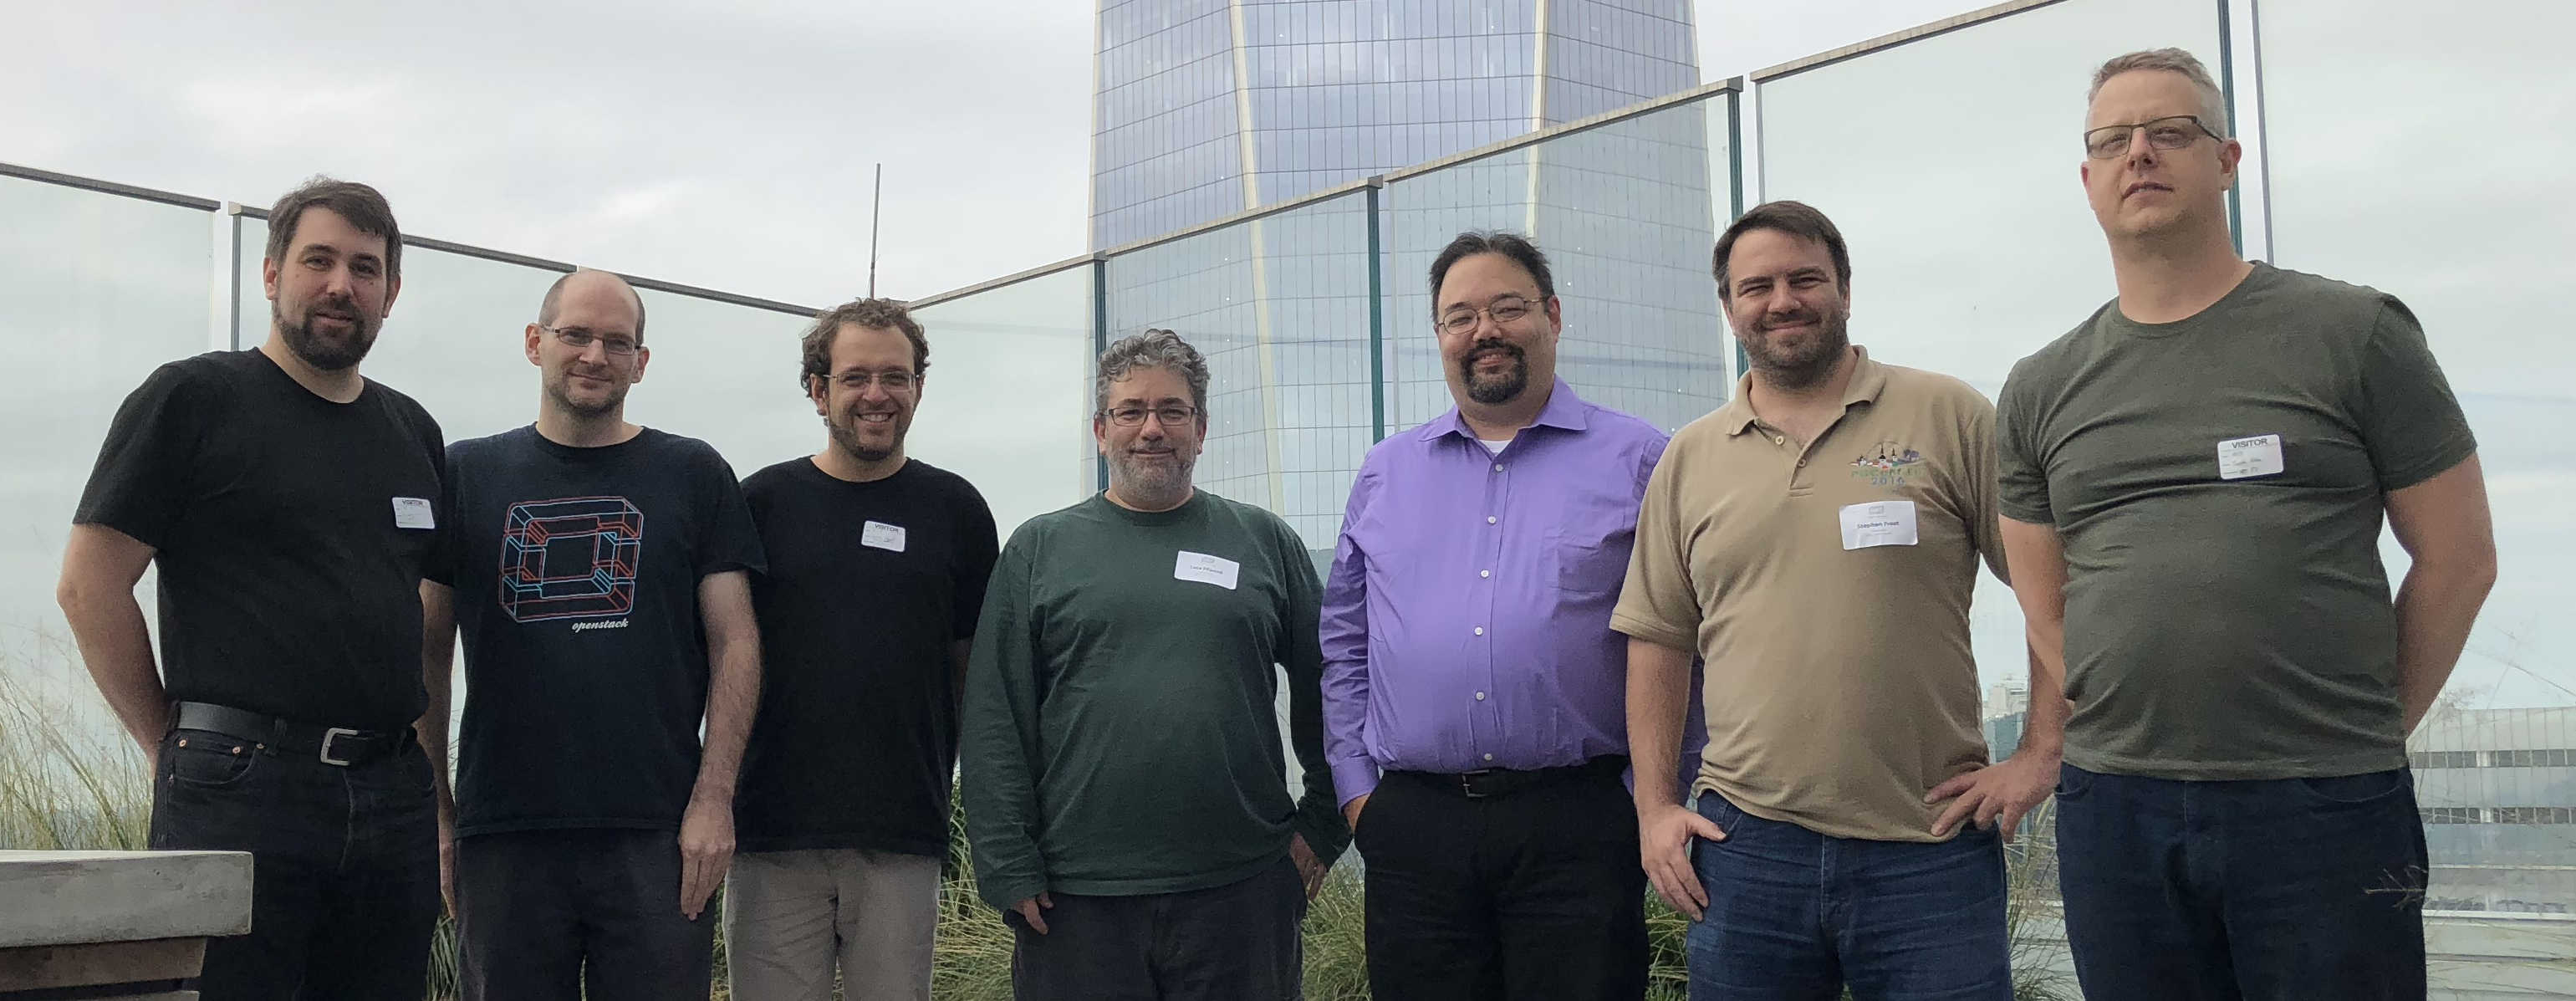
\includegraphics[scale=0.14]{images/2018-october-f2f}

\caption{Face-to-face meeting in New York (October 2018): Martin
Zobel-Helas, Martin Michlmayr, Jimmy Kaplowitz, Luca Filipozzi, Michael
Schultheiss, Stephen Frost, and Tim Potter (left to right)}

\end{figure*}

\chapter{Treasury Report}

This report uses a cash-based method of accounting, recording donations
when deposited (not when the check was written or received by us) and
recording expenses when sent or scheduled for payment (not when
incurred).

\section{Income Statement}

This covers the Period January 1, 2018 -- December 31, 2018

\begin{verbatim}
TODO
\end{verbatim}

\section{Balance Sheet}

\begin{verbatim}
TODO
\end{verbatim}

\chapter{Member Project Reports}

\section{New Associated Projects}

SPI added no new associated projects during 2018.

\section{Projects No Longer Associated with SPI}

\section{Updates from Associated Projects}


\appendix
\chapter{About SPI}

SPI is a non-profit organization which was founded to help organizations
develop and distribute open hardware and software. We encourage programmers
to use the GNU General Public License or other licenses that allow free
redistribution and use of software, and hardware developers to distribute
documentation that will allow device drivers to be written for their product.

SPI was incorporated as a non-profit organization on June 16, 1997 in the state
of New York. Since then, it has become an umbrella organization for projects
from the community.

In 1999, the Internal Revenue Service (IRS) of the United States government
determined that under section 501 (a) of the Internal Revenue Code SPI
qualifies for 501 (c) (3) (non-profit organization) status under section 509
(a) (1) and 170 (b) (1) (A) (vi). This means that donations made to SPI and its
supported projects should be tax deductible for the American donor.

\newpage

\pagestyle{empty}

\backgroundsetup{
scale=1,
angle=0,
opacity=1,
% FIXME: update for 2018
contents={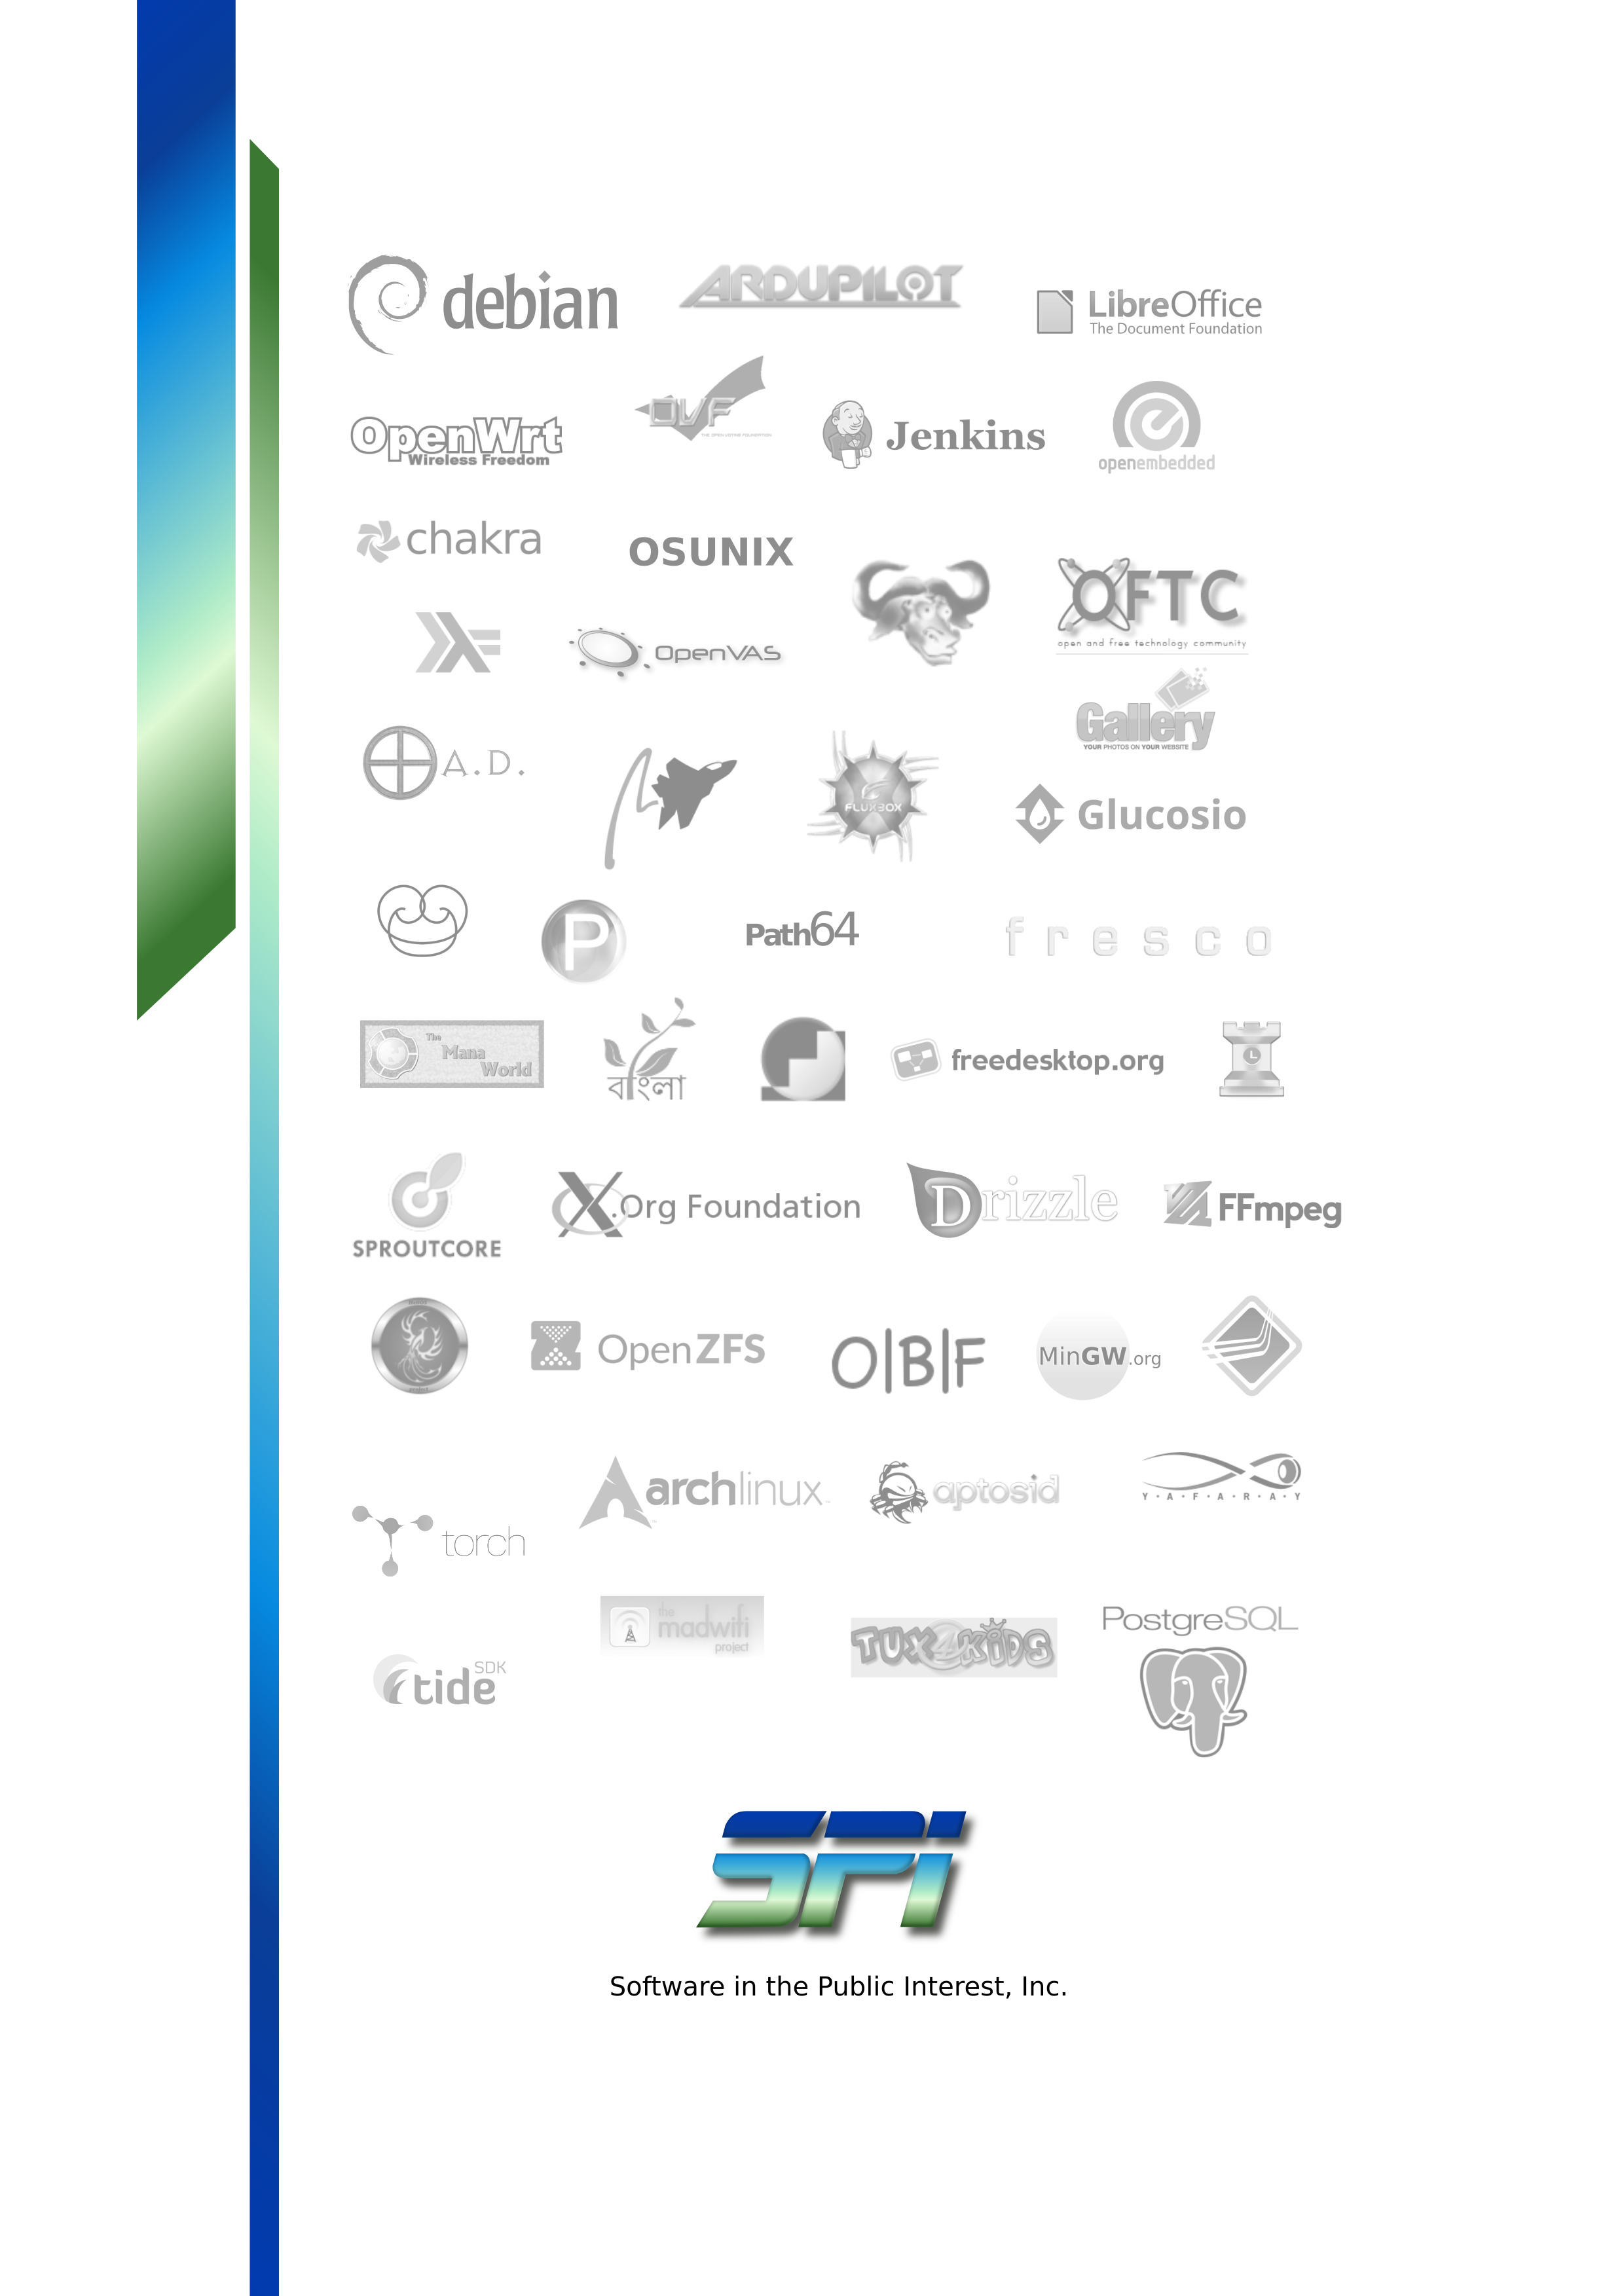
\includegraphics[width=\paperwidth,height=\paperheight]{images/spi-back-2017.jpg}}
}

\null

\end{document}
% Keep this at the bottom, thanks.
% Local Variables:
% TeX-master: "report"
% End:
